\begin{table}[htbp]
\centering
\caption{Especificações de projeto do conversor Buck \Interleaved de dois ramos}
\label{tab:treinamento-dataset}
\begin{tabular}{@{}|m{0.25\textwidth}|m{0.25\textwidth}|m{0.25\textwidth}|@{}}
\hline
\textbf{Tipo do Defeito} & \textbf{Número de Imagens} & \textbf{Quantidade Total de Defeitos} \\
\hline
Falta de Estanho    & 115   & 497 \\
Falta de Cobre      & 115   & 492 \\
Circuito Aberto     & 116   & 482 \\
Curto-Circuito      & 116   & 491 \\
Excesso de Cobre    & 115   & 488 \\
Trilha Desconectada & 116   & 503 \\
\hline
\end{tabular}
\indentedfont[0.96\textwidth]{\citeonline{ref:Huang-et-al}}
\end{table}

\begin{figure}[h!]
    \centering
    \caption{Exemplos de funções utilizadas para operação de \textit{pooling}.}
    \begin{subfigure}[H]{\textwidth}
        \centering
        \caption{\textit{Pooling} Médio}
        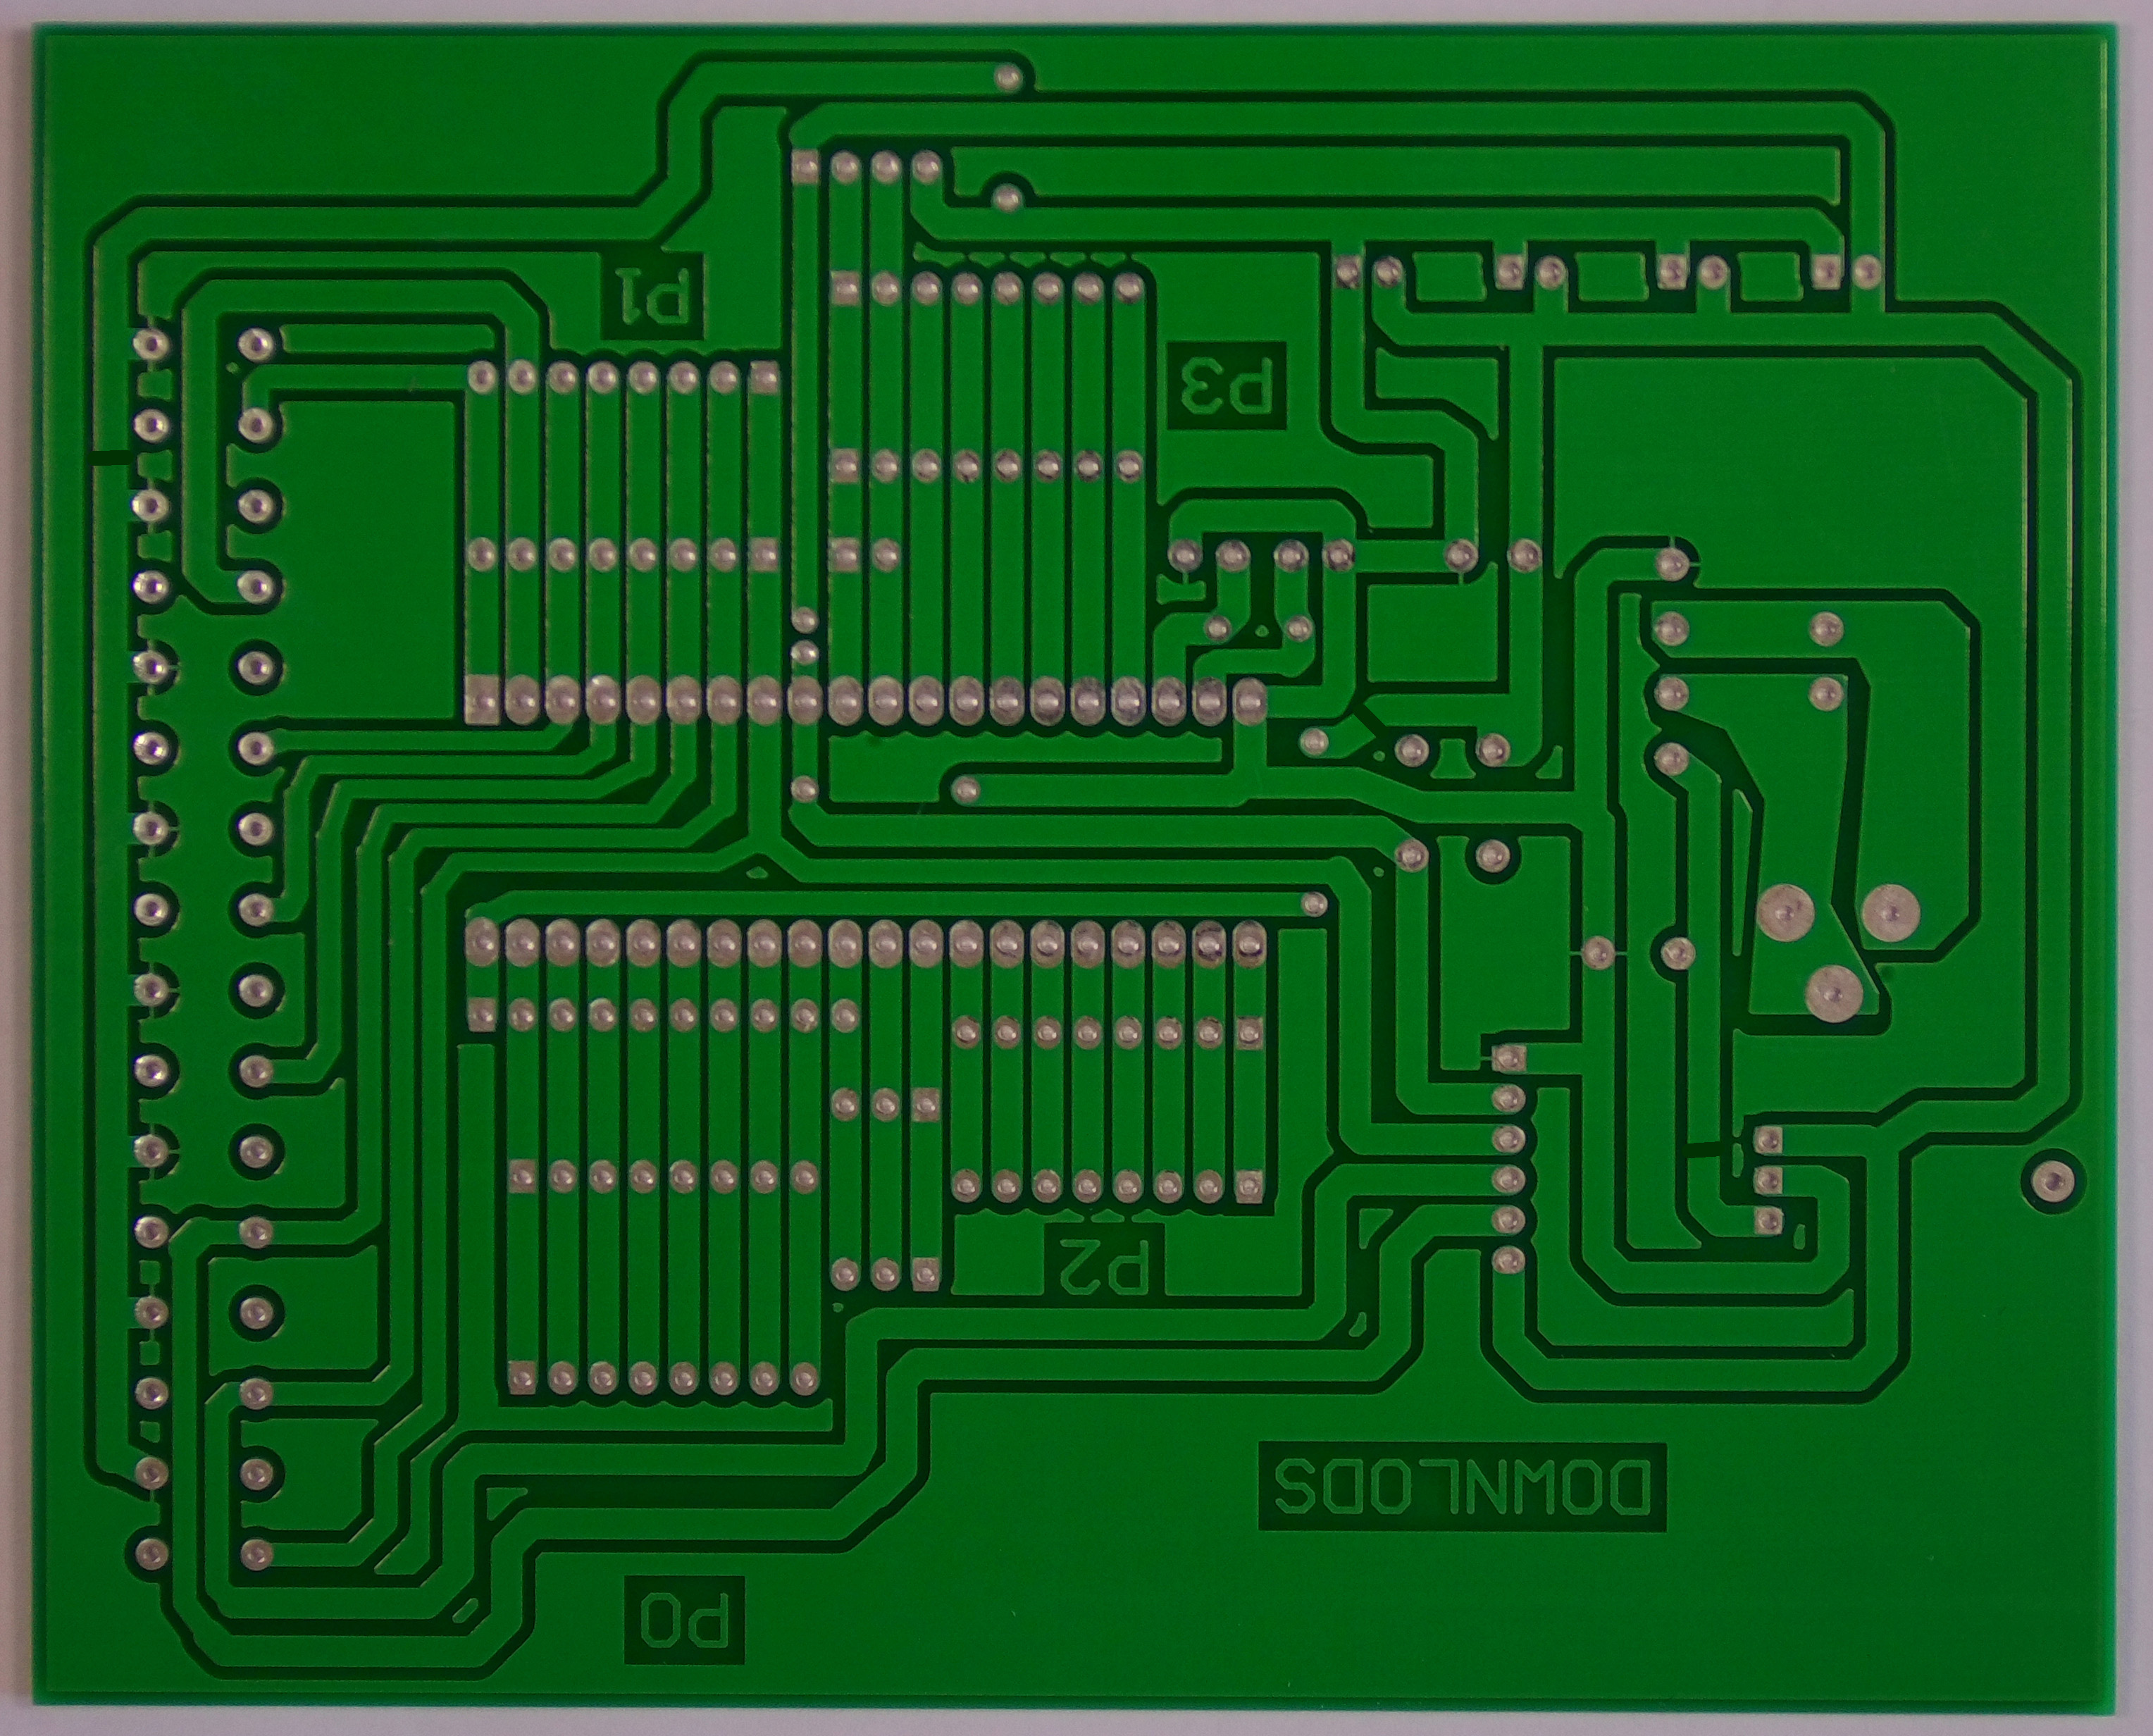
\includegraphics[scale=0.08]{img/img-resultados-hripcb-aberto.jpg}
        \label{fig:resultados-hripc-1}
    \end{subfigure}
    \begin{subfigure}[H]{\textwidth}
        \centering
        \caption{\textit{Max-Pooling}}
        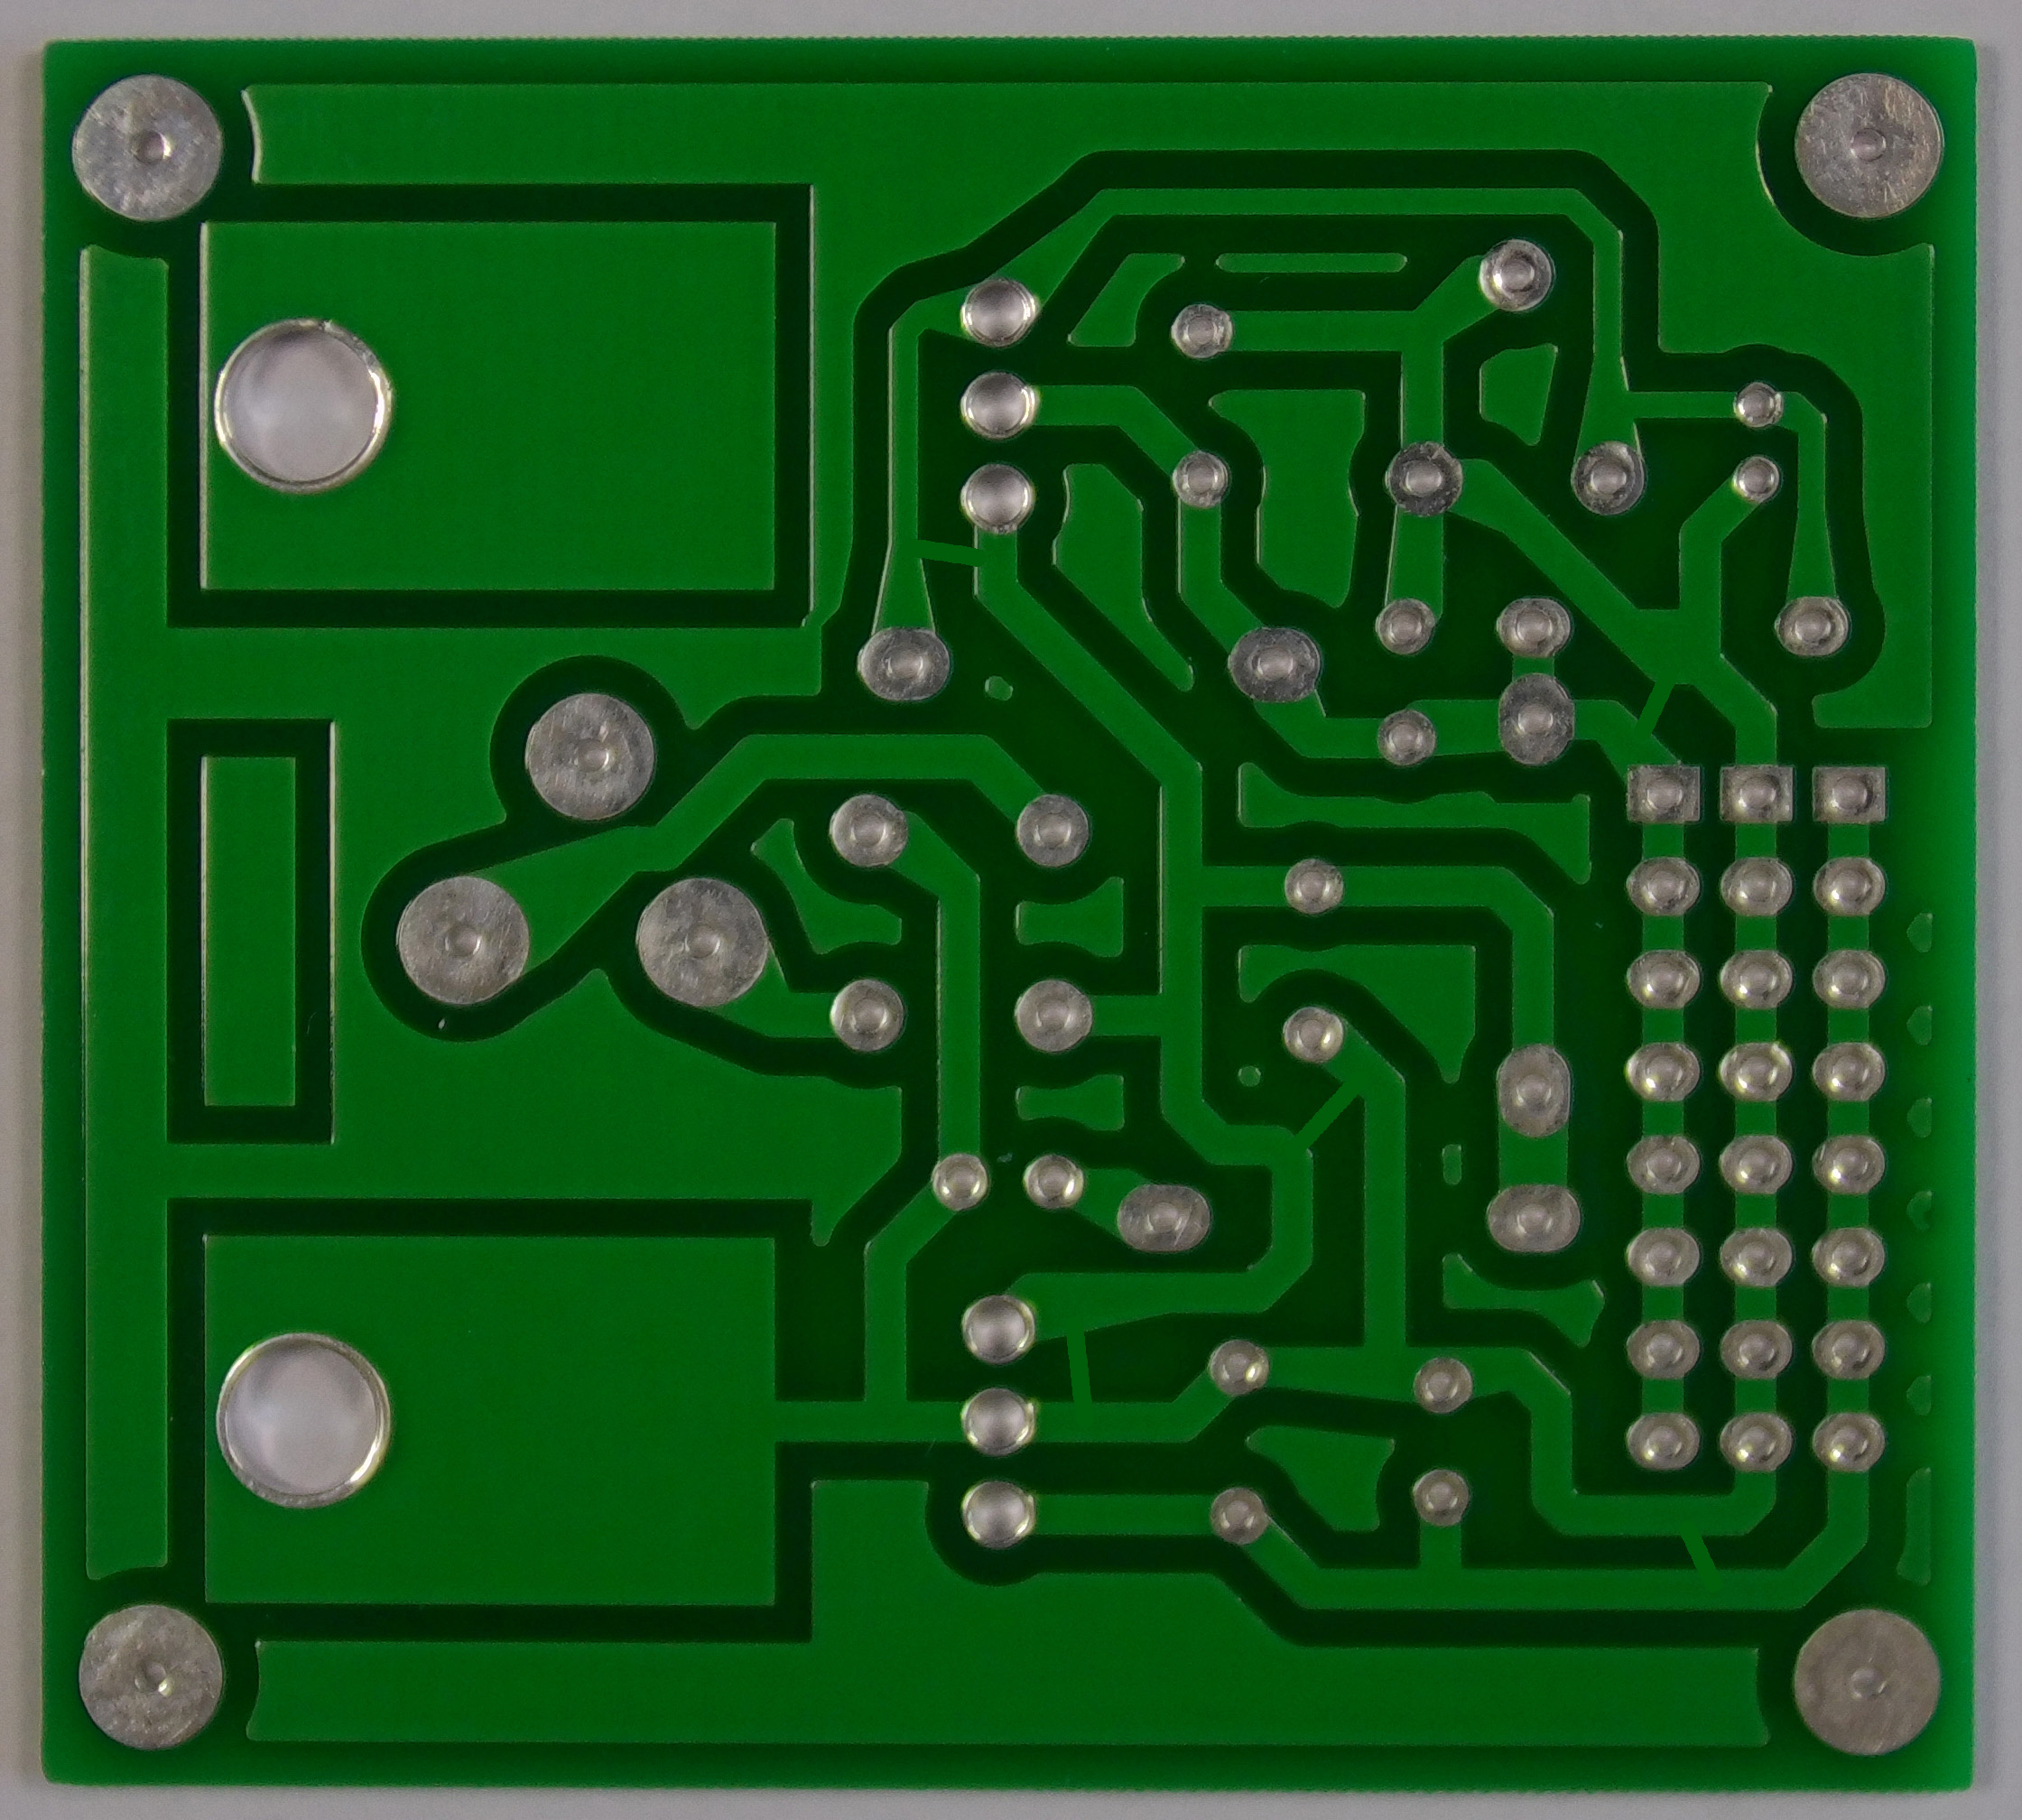
\includegraphics[scale=0.08]{img/img-resultados-hripcb-curto.jpg}
        \label{fig:resultados-hripc-2}
    \end{subfigure}
    \indentedfont[15.5cm]{Adaptado de \citeonline{ref:Gholamalinezhad-Khosravi}}
    \label{fig:resultados-hripc}
\end{figure}
